\chapter{Results}
\label{chapter-results}

Various models were tried using our application. The results were then compared to the existing ones from the CROCS research. We started with simple models from \texttt{scikit} library and smaller datasets (of around 65000 samples). We were able to reach accuracy ranging from 7.5 - 33.5 \% on average (comparable to \cite{thesis_sekan}):

\begin{figure}[H]

\centering

\begin{tabular}{|l|l|}
\hline 
Classifier & $\sim$ accuracy \\
\hline 
RadiusNeighborsClassifier & 7.50 \% \\
QuadraticDiscriminantAnalysis & 7.68 \% \\
ExtraTreeClassifier & 12.62 \% \\
MLPClassifier & 12.65 \% \\
DecisionTreeClassifier & 12.71 \% \\
KNeighborsClassifier & 16.92 \% \\
SGDClassifier & 20.70 \% \\
PassiveAggressiveClassifier & 21.72 \% \\
AdaBoostClassifier & 22.34 \% \\
GaussianNB & 27.51 \% \\
MultinomialNB & 28.22 \% \\
LinearSVC & 29.93 \% \\
LinearDiscriminantAnalysis & 30.81 \% \\
NuSVC & 30.93 \% \\
RidgeClassifier & 31.14 \% \\
BernoulliNB & 31.21 \% \\
RidgeClassifierCV & 31.22 \% \\
SVC & 32.57 \% \\
BaggingClassifier & 32.74 \% \\
RandomForestClassifier & 33.04 \% \\
ExtraTreesClassifier & 33.26 \% \\
GradientBoostingClassifier & 33.57 \% \\ 
\hline
\end{tabular}

\end{figure}

\section{Multi layer perceptrons}

Before any models were trained, we performed an analysis of the dataset, applied feature engineering and extracted the features described in the subsection \ref{feature-engineering}. We took the whole key (as a binary vector of respective key length 512 / 1024 / 2048) and all its moduli up to 30. Modulus was also represented as a binary vector. For example, the feature modulo 7 could result in 6 different vectors, each having a different index set to 1 and representing one of 6 possible remainders. In the end, we obtained one large binary vector which we fed to the models.

\subsection*{Grid search}

Apart from the features extracted from the analysis, all the other tried features seem to have a uniform distribution within its domain. On the first look, the model to be used is not apparent, so we decided to use the \textbf{grid search}\footnote{described in section \ref{section-grid-search}} for finding the most suitable topology and configuration. 

We used this approach mainly to find the optimal choice of the topology (meaning the number of hidden layers and the number of neurons within each layer), the selected activations in each layer and optimizers.

We were gradually testing topologies from zero up to two hidden layers, with the number of neurons being the powers of 2 starting from 8 up to 4096. The activation functions used were sigmoid, hyperbolic tangent, ReLU and leaky ReLU. This gives us around 160 different configurations to run, which is an ideal use case for cloud computing. Running for a couple of days, we were able to compare all these different configurations on the same datasets.

As for the activation, the usage sigmoid resulted in lower overall accuracy (36.95 \% - 41.89 \%). Hyperbolic tangent and ReLU performed better (36.3 \% - 42.29 \% for tanh and 37.26 \% - 42.46 \% for ReLU), presumably because they are centered in 0. With different optimizers, the differences were negligible. In the end, we chose Adam optimizer. In conclusion, the choice of activation nor the optimizer did not rapidly impact the overall accuracy. 

The choice of topology affected the accuracy more significantly. The sparse models with the lower number of neurons in the hidden layers (less than 32) performed worse (less than or around 40 \%). When adding the layer with at least one dense layer of 256+ neurons, the models usually reached the accuracy of up to 42 \%, no matter the activation or the optimizer.

\subsection*{Training fine-tuning}

We generated our training / valid and test data in the ratio of 60:20:20. All of these sets were disjoint. Training and validation sets were used during the training phase and the independent test set for the final evaluation and overall accuracy. However, even if the overall accuracy reached 40 \%, it happened, that the classifier was poorly trained, especially when the probability distribution of labels over the training set was not uniform. The huge class 13 overshadowed all the other classes. Based on the confusion matrix, we replicated the inferior entries in the training data to obtain uniform distribution. Experimenting with different uniform datasets, we set the optimal number of training epochs to 4. In the later epochs, the models were already overfitting the training data.

Given this adjustments, we were able to train models to perform with an overall accuracy of more than 43 \%. In the figure \ref{comparison-results} we can see the comparison of the CROCS results and our model. Accuracy table consists of rows representing the individual groups, the bigger columns saying whether the group correctly classified within the top 1 (2, 3) results from the classifier and the smaller columns saying how many keys were used by the neural network. We can see that on some groups (like groups 6, 9, 11, 12, 13) it performed better than the previous classifier. On the other hand, it struggled with group 4.

The model had one hidden layer of 256 ReLU neurons, the output layer with softmax activation and used categorical cross-entropy for a loss function. The training dataset had more than 1 million keys, with validation and test data of around 350 thousand keys. The model took around 2 hours to train on Metacentrum.

\begin{sidewaysfigure}[htbp]

\centering
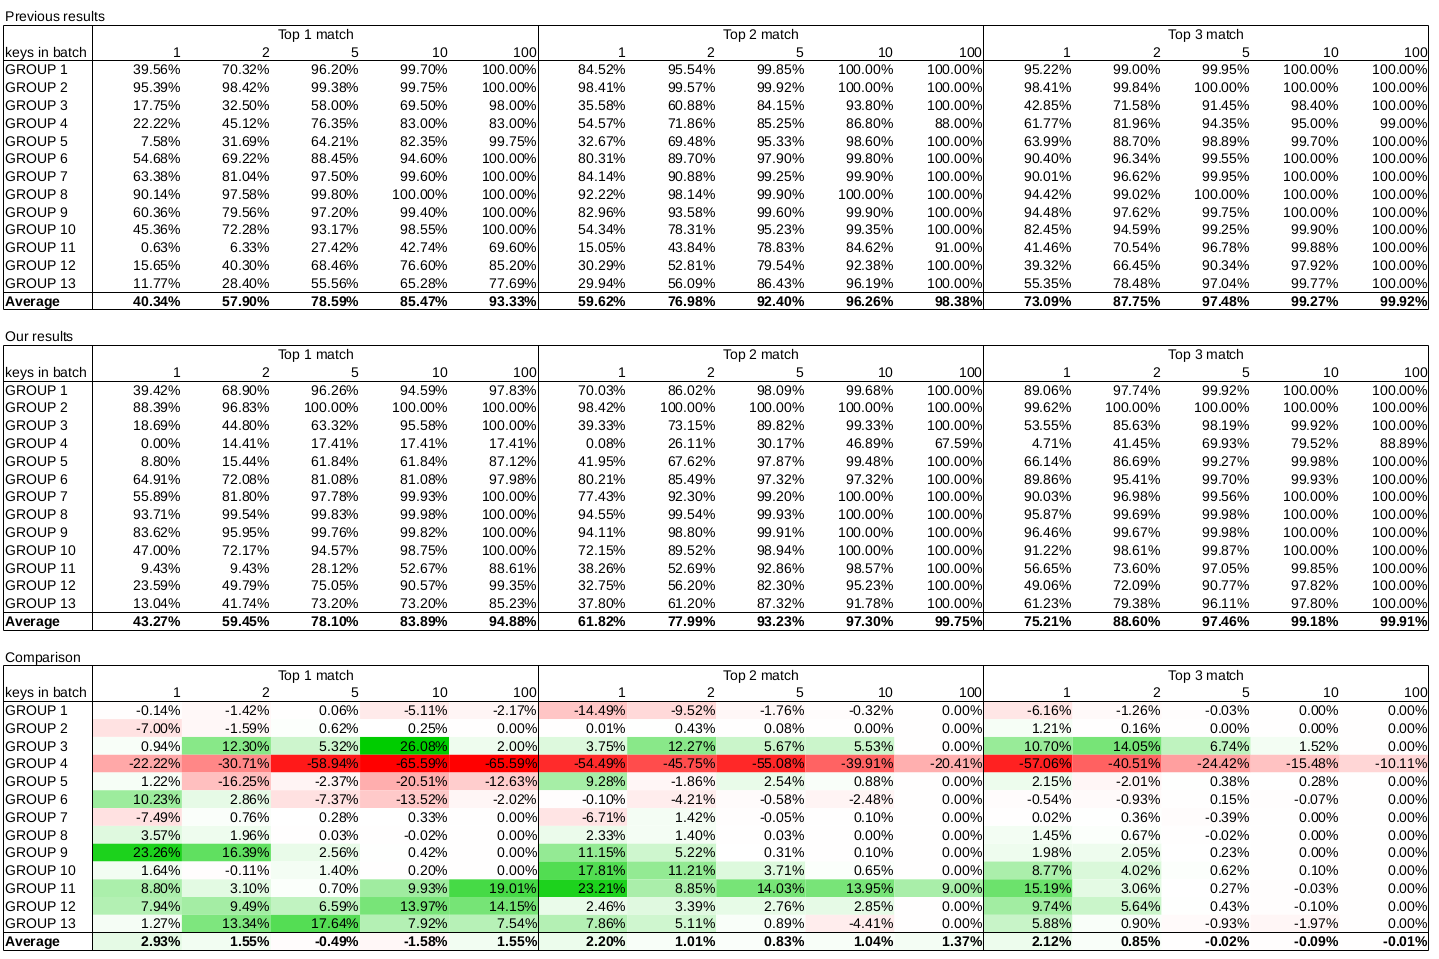
\includegraphics[width=\textwidth]{tex/images/results/comparison_13}
\caption{Comparison of results of CROCS lab and our model.}
\label{comparison-results}

\end{sidewaysfigure}

\noindent
When comparing the Naive Bayes model and the optimized neural network we can see, that:

\begin{itemize}

\item neural network model was able to adapt to the more complex dataset, when compared to the scikit models. That is why the best-evaluated scikit model lags behind simple keras classifiers in accuracy.

\item our classifier was able to increase the overall accuracy by almost 3 \% when compared to the methods used by CROCS lab and almost 10 \% when compared to the best results achieved in \cite{thesis_sekan}.

\item a neural network is substantially better in classifying Group 9 (Yubikey 1 \& Infineon JTOP 80K). Given the recent problems with Infineon keys \cite{svenda_2}, discovering their keys with high probability could have been used for potential attack.

\item it performs slightly better on groups 8, 10, 11, 12, 13. 

\item when using a batch of 10+ keys, it can better differentiate groups 11, 12, beating Naive Bayes by 15 - 19 \% (group 11 contains very popular libraries like Crpyto++ and Microsoft crypto libraries).

\item when using a batch of 5+ keys, it can better differentiate group 13 beating Naive Bayes by 17.64 \% with accuracy 73.2 \%. The group 13 contains the highest number of sources, so the bigger success rate applies to a bigger set of sources.

\item the network has really struggled with the group 4. The main reason may have been insufficient data for this group (around 50K for 1024b and 200K for 512b). Therefore it was difficult to generate a balanced dataset containing this group.

\end{itemize}

\subsection*{Binary classifiers}

Based on the previous general model results we can see, that some groups can be detected with high probability even using one single key. We tried to train binary classifiers to differentiate these classes better:

\begin{figure}[H]

%first line
\begin{subfigure}{.33\textwidth}
  \centering
  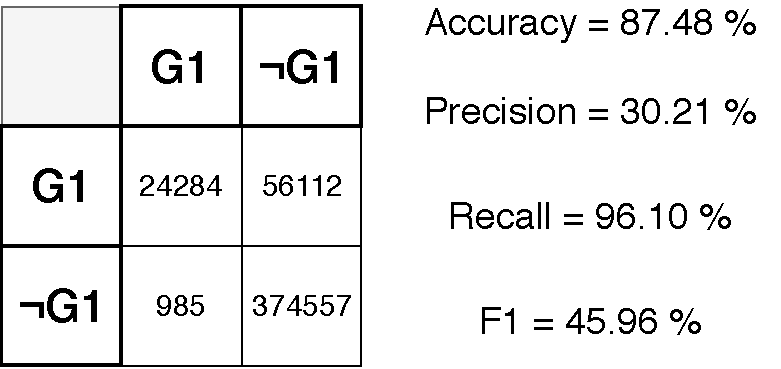
\includegraphics[width=\textwidth]{tex/images/results/rese_g1_512}  
\end{subfigure}%
\begin{subfigure}{.33\textwidth}
  \centering
  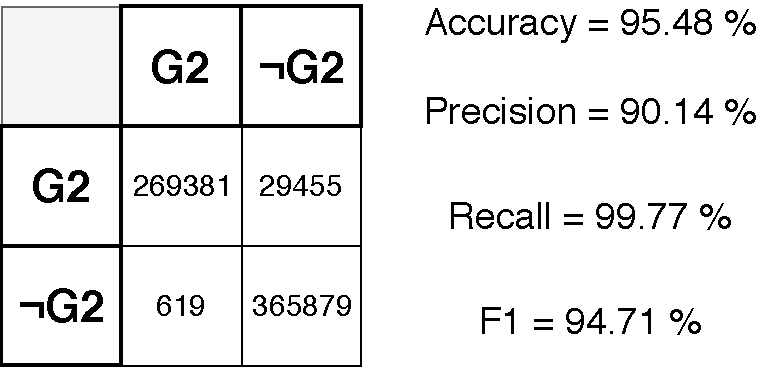
\includegraphics[width=\textwidth]{tex/images/results/rese_g2_512}
\end{subfigure}
\begin{subfigure}{.33\textwidth}
  \centering
  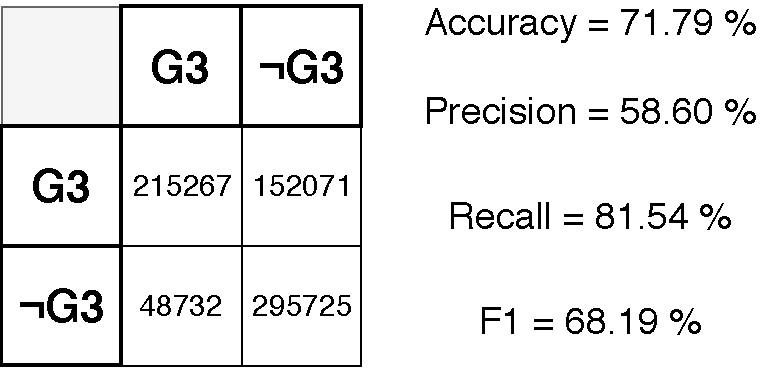
\includegraphics[width=\textwidth]{tex/images/results/rese_g3_512}
\end{subfigure}

\vspace{3mm}
%second line
\begin{subfigure}{.33\textwidth}
  \centering
  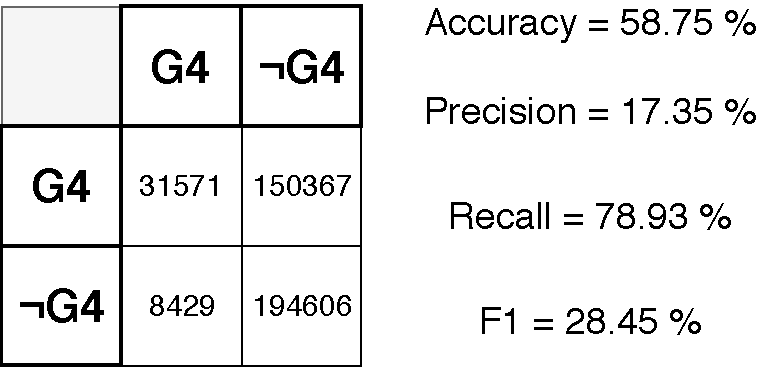
\includegraphics[width=\textwidth]{tex/images/results/rese_g4_512}  
\end{subfigure}%
\begin{subfigure}{.33\textwidth}
  \centering
  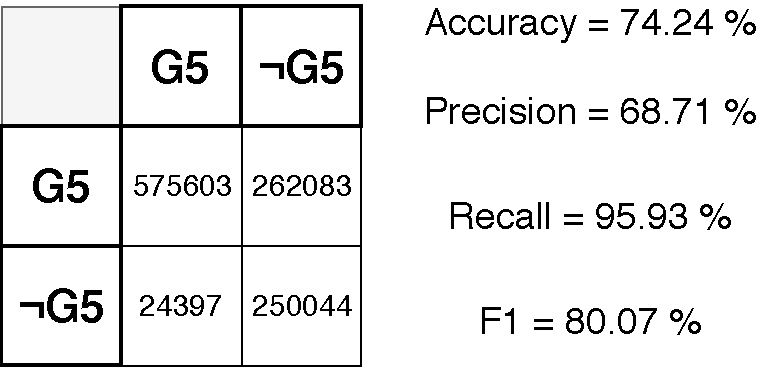
\includegraphics[width=\textwidth]{tex/images/results/rese_g5_512}
\end{subfigure}
\begin{subfigure}{.33\textwidth}
  \centering
  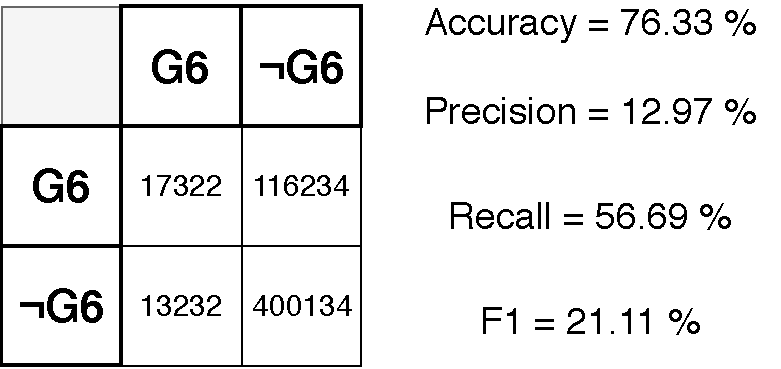
\includegraphics[width=\textwidth]{tex/images/results/rese_g6_512}
\end{subfigure}

\vspace{3mm}
%third line
\begin{subfigure}{.33\textwidth}
  \centering
  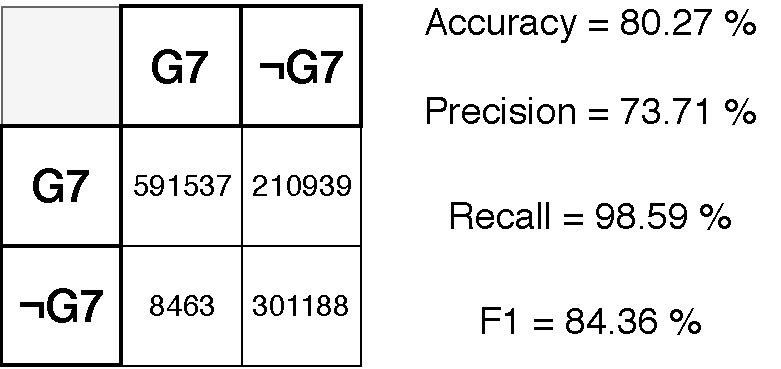
\includegraphics[width=\textwidth]{tex/images/results/rese_g7_512}  
\end{subfigure}%
\begin{subfigure}{.33\textwidth}
  \centering
  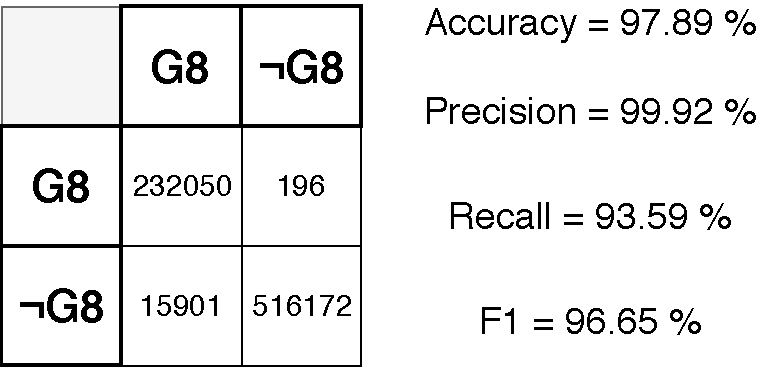
\includegraphics[width=\textwidth]{tex/images/results/rese_g8_512}
\end{subfigure}
\begin{subfigure}{.33\textwidth}
  \centering
  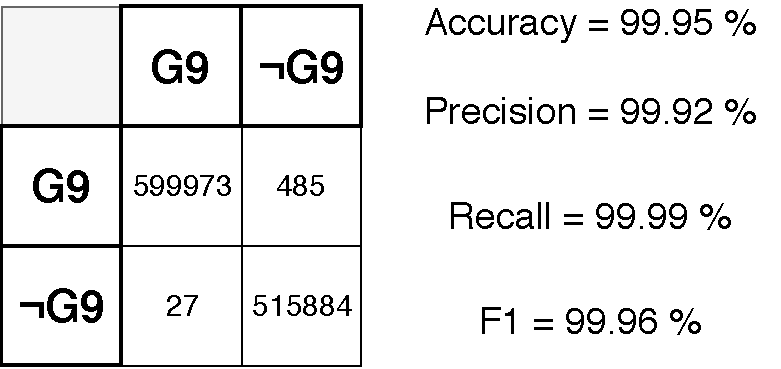
\includegraphics[width=\textwidth]{tex/images/results/rese_g9_512}
\end{subfigure}

\vspace{3mm}
%fourth line
\begin{subfigure}{.33\textwidth}
  \centering
  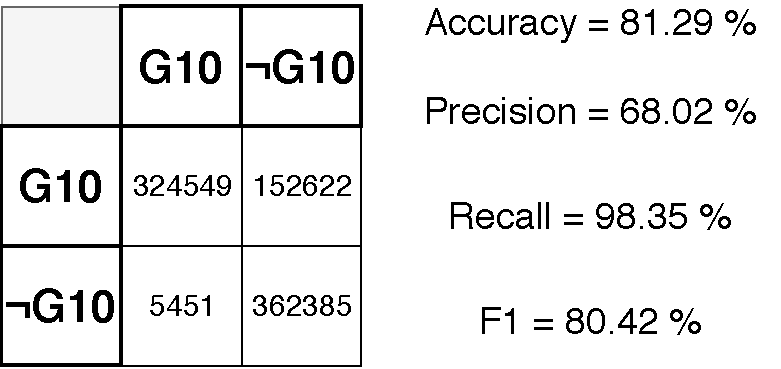
\includegraphics[width=\textwidth]{tex/images/results/rese_g10_512}  
\end{subfigure}%
\begin{subfigure}{.33\textwidth}
  \centering
  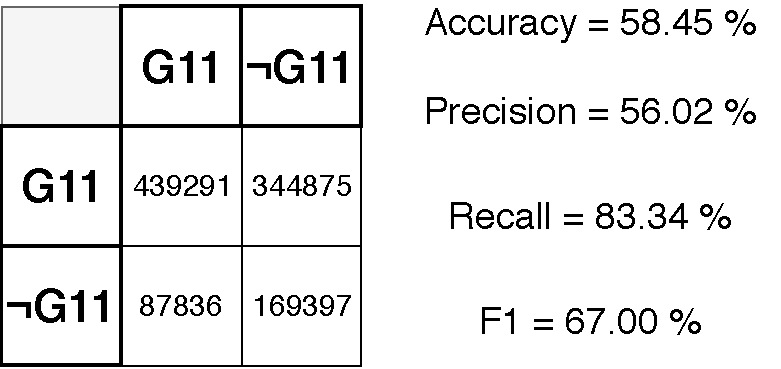
\includegraphics[width=\textwidth]{tex/images/results/rese_g11_512}
\end{subfigure}
\begin{subfigure}{.33\textwidth}
  \centering
  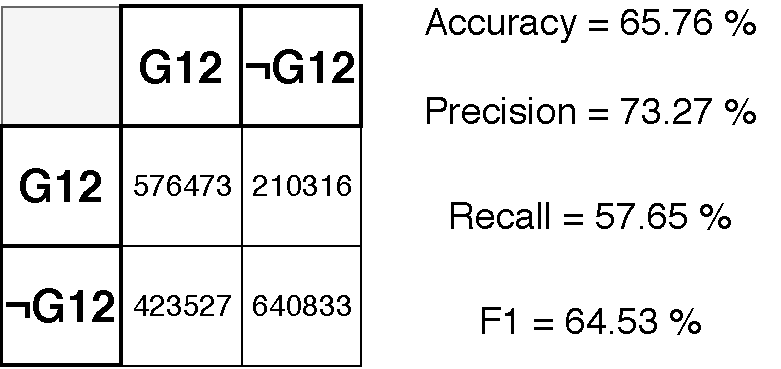
\includegraphics[width=\textwidth]{tex/images/results/rese_g12_512}
\end{subfigure}

\vspace{3mm}
%last line
\begin{subfigure}{.33\textwidth}
  \centering
  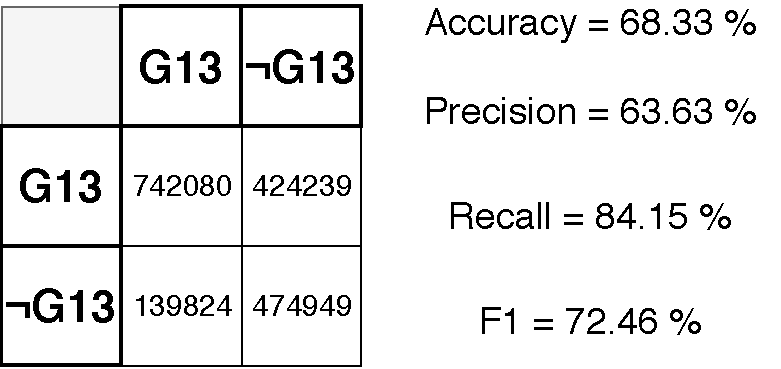
\includegraphics[width=\textwidth]{tex/images/results/rese_g13_512}  
\end{subfigure}%

\caption{Confusion matrices and metrics for 13 classifiers for each group trained individually.}

\end{figure}

\noindent
These results are comparable to the observations from the previous trial:

\begin{itemize}

% \item the network completely fails to detect group 4 (even worse than random guessing)
\item it is more or less equal to random guessing when detecting group 11
\item groups 1, 3, 4, 5, 6, 7, 10, 11 and 13 have lower precision leading to the higher number of false positives
\item the results for the biggest groups 7, 12 and 13 are more promising. It shows, that we can differentiate them better with accuracy and precision above 65 to 70 \%
\item we obtained good results for group 2, 8 and 9 given their strong distribution imprint over selected features
\item group 9 is detected very reliably having less than 0.1 \% chance of incorrect classification

\end{itemize}

Given the fact that every classifier can be trained individually, we obtained the best results when putting them all together in the voting process. The same input was fed to 13 different binary classifiers, that outputted the probability, that the key belongs to the respective group. The classifier with the highest probability was voted as a winner.

We ran the voting classifier on the uniformly distributed dataset of 13 groups of bit length 1024. Table \ref{table-binary-voter} shows the obtained results. The notable observations of this run are:

\begin{itemize}

\item the overall accuracy is still higher than naive Bayes

\item the classifier struggles with insufficient datasets for groups 1 and 6 where it is remarkably worse than naive Bayes

\item it gets more successful in identifying large groups, especially groups 7, 12 and 13. Given the fact, that these groups produce the majority of keys on the internet makes this result more significant

\item as expected from the confusion matrix, the classifier is reliable in recognizing the group 9 with almost 40 \% improvement over naive Bayes\footnote{Group 9 contains Infineon chips, which were liable to attack as reported in \cite{svenda_2}. The correct classification of such group could be useful for the potential attacker.}

\end{itemize}

\begin{table}[h]
\centering
\begin{tabular}{| r | c | c | c |}
\hline
Group & Top 1 match                     & Top 2 match                     & Top 3 match                     \\
\hline
1     & 45.23 \% {\color[HTML]{9B9B9B} (39.56 \%)} & 60.10 \% {\color[HTML]{9B9B9B} (84.52 \%)} & 87.87 \% {\color[HTML]{9B9B9B} (95.22 \%)} \\

2     & 70.79 \% {\color[HTML]{9B9B9B} (95.39 \%)} & 95.54 \% {\color[HTML]{9B9B9B} (98.41 \%)} & 99.29 \% {\color[HTML]{9B9B9B} (98.41 \%)} \\

3     & 18.71 \% {\color[HTML]{9B9B9B} (17.75 \%)} & 41.58 \% {\color[HTML]{9B9B9B} (35.58 \%)} & 55.79 \% {\color[HTML]{9B9B9B} (42.85 \%)} \\

4     & 34.08 \% {\color[HTML]{9B9B9B} (22.22 \%)} & 58.88 \% {\color[HTML]{9B9B9B} (54.57 \%)} & 74.88 \% {\color[HTML]{9B9B9B} (61.77 \%)} \\

5     & 8.59 \% {\color[HTML]{9B9B9B}( 7.58 \%)}  & 30.64 \% {\color[HTML]{9B9B9B} (32.67 \%)} & 58.31 \% {\color[HTML]{9B9B9B} (63.99 \%)} \\

6     & 23.44 \% {\color[HTML]{9B9B9B} (54.68 \%)} & 43.44 \% {\color[HTML]{9B9B9B} (80.31 \%)} & 55.55 \% {\color[HTML]{9B9B9B} (90.40 \%)} \\

7     & 78.14 \% {\color[HTML]{9B9B9B} (63.38 \%)} & 93.75 \% {\color[HTML]{9B9B9B} (84.14 \%)} & 96.62 \% {\color[HTML]{9B9B9B} (90.01 \%)} \\

8     & 93.53 \% {\color[HTML]{9B9B9B} (90.14 \%)} & 93.69 \% {\color[HTML]{9B9B9B} (92.22 \%)} & 94.54 \% {\color[HTML]{9B9B9B} (94.42 \%)} \\

9     & 99.77 \% {\color[HTML]{9B9B9B} (60.36 \%)} & 99.97 \% {\color[HTML]{9B9B9B} (82.96 \%)} & 99.99 \% {\color[HTML]{9B9B9B} (94.48 \%)} \\

10    & 45.61 \% {\color[HTML]{9B9B9B} (45.36 \%)} & 83.81 \% {\color[HTML]{9B9B9B} (54.34 \%)} & 94.68 \% {\color[HTML]{9B9B9B} (82.45 \%)} \\

11    & 0.94 \% {\color[HTML]{9B9B9B}( 0.63 \%)}  & 19.87 \% {\color[HTML]{9B9B9B} (15.05 \%)} & 50.01 \% {\color[HTML]{9B9B9B} (41.46 \%)} \\

12    & 24.21 \% {\color[HTML]{9B9B9B} (15.65 \%)} & 30.75 \% {\color[HTML]{9B9B9B} (30.29 \%)} & 41.90 \% {\color[HTML]{9B9B9B} (39.32 \%)} \\

13    & 21.81 \% {\color[HTML]{9B9B9B} (11.77 \%)} & 49.36 \% {\color[HTML]{9B9B9B} (29.94 \%)} & 64.19 \% {\color[HTML]{9B9B9B} (55.35 \%)} \\

\hline
TOTAL & 41.12 \% {\color[HTML]{9B9B9B} (40.34 \%)} & 59.82 \% {\color[HTML]{9B9B9B} (59.62 \%)} & 73.36 \% {\color[HTML]{9B9B9B} (73.09 \%)} \\
\hline                       
\end{tabular}
\caption{Accuracy table for a voting classifier of binary classifiers.}
\label{table-binary-voter}
\end{table}

The voting classifier performs better than the previous one when classifying big groups. Looking at the precisions of the individual groups, one can combine the results of all of the three existing classifiers to obtain more accurate predictions.

\subsection*{Group spliting}

As the last step, we tried even more precise classification between sources. We aimed to split at least one of the 13 groups. In the first approach, we ran the models on the huge dataset with 64 individual sources. In the second one, we took sources only from a single group and tried to classify them within it. We repeated it for each group.

However, when running several proven models on each group, the results showed as expected the uniform distribution in classification within the group, as the sources in one group shared the same distribution on the features. The network is not able to differentiate between them and is performing with the same results as random guessing. We suppose that the sources within each group share the same implementation steps that affect the distribution on bits in the public key and the distribution on the remainders modulo up to 30.

